\chapter{Testautomatisierung mit Selenium}
\label{sec:testautomatisierung_mit_selenium}

Laut Seidel et al. \cite[vgl. S. 48]{seidl_basiswissen_2012} ist der am häufigsten genutzte \frqq Angriffspunkt\flqq\ für Testautomatisierung die grafische Benutzerschnittstelle. Seidel et al. \cite[S. 48]{seidl_basiswissen_2012} nennen dafür folgende Gründe:
\begin{itemize}
\item \glqq Sie ist für Tester und Automatisierer anschaulich und leicht greifbar.\grqq
\item \glqq Sie stellt zumeist das Verhalten im realen Umfeld am besten nach.\grqq
\item \glqq Die Dokumentation von Systemen ist auf dieser Ebene meist am vollständigsten.\grqq
\item \glqq Der klassische Systemtest wird oft über diese Schnittstelle abgewickelt.\grqq
\item \glqq Hinter der grafischen Benutzerschnittstelle liegende Systeme werden implizit getestet.\grqq
\end{itemize}
Ein großer Teil der heutzutage entwickelten Anwendungen werden in Form einer Webapplikation realisiert. Für automatisierte Testfälle, die als Schnittstelle die grafische Benutzeroberfläche verwenden, stellen diese Webapplikation einen Sonderfall dar. Elemente auf der Oberfläche können besonders gut angesprochen werden.
Im Gegensatz zu gewöhnlichen Desktopanwendungen gibt es bei dieser Art von Anwendung, wie Seidel et al. \cite[vgl. S. 88]{seidl_basiswissen_2012} feststellen, \glqq keinen spezifischen Client für eine Applikation, sondern einen generischen - den Browser.\grqq\ Dieser schafft nach Seidel et al.  \cite[vgl. S. 59]{seidl_basiswissen_2012} für Werkzeuge eine sehr  gute Basis, um auf Elemente der Seite zuzugreien. Die einzelnen HTML-Elemente und deren Attribute können verwendet werden, um die Bestandteile einer Seite zu adressieren.
Ein weit verbreitetes Tool für die Automatisierung, welches diesen Ansatz verfolgt, ist Selenium \cite{selenium_selenium_2015}.
\section{Selenium}
\label{sec:selenium}
Seidel et al. \cite[S. 142]{seidl_basiswissen_2012} beschreiben Selenium als \glqq eines der gängigsten Open-Source-Automatisierungswerkzeuge für Webapplikationen.\grqq\\
Ordnet man Selenium, der in Kapitel \ref{subsec:testcodeerstellung} erstellten Unterteilung in der Testcodeerstellung zu, ist dieses im unteren mittleren und unteren linken Quadranten angesiedelt. Abbildung \ref{fig:bereicheTestcodeerstellungSelenium} hinterlegt diese Bereiche farblich.
Selenium ist also ein Tool, mit welchem Testfälle erstellt werden können, die als Schnittstelle die grafische Benutzeroberfläche eine Webanwendung verwenden. Die Testcodeerstellung erfolgt dabei manuell oder teilautomatisiert mittels \grq record-and playback\grq.\\

\begin{figure}[htb]
  \centering  
  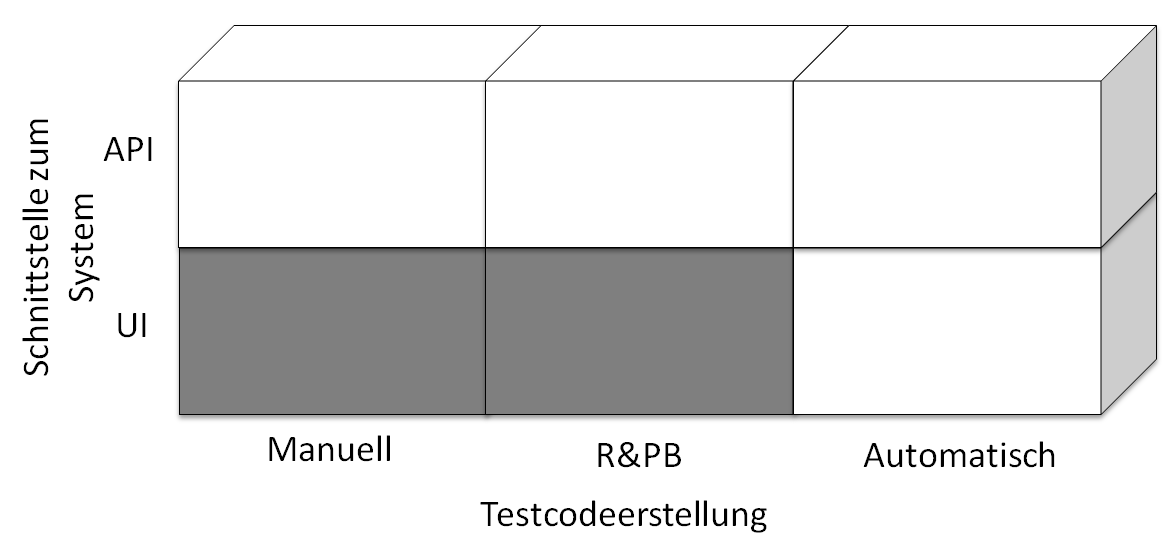
\includegraphics[scale=0.7]{img/bereicheTestcodeerstellungSelenium.png}\\
  \footnotesize\sffamily\textbf{Quelle:} vgl. \cite{meszaros_agile_2003}
  \caption{Einordnung von Selenium in die verschiedene Möglichkeiten der Testcodeerstellung}
  \label{fig:bereicheTestcodeerstellungSelenium}
\end{figure}

Selenium besteht nicht nur aus einem einzelnen Tool, sondern aus einer Vielzahl an Tools, die unter dem Namen \grq Selenium\grq\ zusammengefasst werden.
In seiner aktuellen Ausprägung 2.48 lassen sich, abgesehen von Komponenten die der Abwärtskompatibilität dienen, laut Dokumentation \cite{selenium_selenium_2015-1}, drei Komponenten unterscheiden:

\begin{itemize}
\item Selenium IDE \\
Bei der Selenium IDE handelt es sich um ein Firefox plug-in, das verwendet werden kann, um Selenium-Testscripte zu erstellen. Testscripte können von Hand erstellt, oder mittels eines \grq record-and playback\grq -Mechanismus direkt im Browser aufgezeichnet werden. Die erstellten Testfälle können mit Akzeptanzkriterien angereichert und innerhalb der IDE wieder abgespielt werden.
\item Selenium WebDriver \\
Der Selenium WebDriver bietet für verschiedene Programmiersprachen eine Schnittstelle zur Steuerung eines Browsers aus dem Programmcode heraus. Der WebDriver bildet damit die Kernkomponente für alle Selenium-Testfälle, die außerhalb der Selenium IDE entwickelt werden.

\item Selenium Server/Grid \\
Mit Hilfe des Selenium Servers ist es möglich, Selenium-Testfälle nicht nur auf dem eigenen Rechner auszuführen, sondern die Ausführung auf einen Server auszulagern. Einen wichtigen Teil des Selenium Server bildet Selenium Grid. Selenium Grid bietet die Möglichkeit, die Ausführung über einen Server hinaus auf eine Vielzahl von Knoten zu verteilen. Der Selenium Server dient dann als Hub, der die Testfallanfragen auf registrierte Knoten zur Ausführung weiterleitet. 
\end{itemize}


\section{Testdurchführung mit Selenium}
\label{sec:testdurchführung_mit_selenium}
Abhängig davon, ob die Testfälle für die Selenium IDE entwickelt wurden, oder sich auf den Selenium WebDriver stützen, unterscheiden sich die Möglichkeiten zur Ausführung der Testskripte.\\
Testfälle, die mit der Selenium IDE entwickelt wurden, verwenden eine eigene Sprache, mit dem Namen \grq Selense\grq.\ Diese Testfälle können in späteren Testläufen wieder über die Selenium IDE zur Ausführung gebracht werden. \\
Dem gegenüber stehen Testfälle, die den Selenium WebDriver verwenden.
Testfälle die mittels Selenium WebDriver entwickelt wurden, sind für ihre Ausführung nicht an ein spezielles Tool gebunden. Beim WebDriver handelt es sich um eine API, mit deren Hilfe ein Browser ferngesteuert werden kann. Die Integration der API wird dem Ersteller selbst überlassen. In der Praxis hat sich als Best Practice herausgestellt, den WebDriver in Verbindung mit einem Unit-Framework einzusetzen.
Im Java-Umfeld wären hier beispielsweise JUnit oder TestNG zu nennen.
Die Testfälle können analog zu den klassischen Unit Tests entwickelt werden, verwenden jedoch als Schnittstelle zum System die Benutzeroberfläche der Webanwendung. 
Die Ausführung erfolgt identisch zu den klassischen Unit Tests.\\
Bei Verwendung des WebDrivers ist Selenium, durch die eingesetzten Unit-Frameworks, in den meisten Programmiersprachen bereits gut in die Infrastruktur integriert. Testfälle in Java, die mittels JUnit ausgeführt werden, sind in allen gängigen IDEs, durch Plugins unterstützt. Große Bedeutung hat auch eine gute Integration in den Buildprozess. Werden in Java Standarttools, wie beispielsweise Gradle oder Maven zum Bauen der Projekte verwendet, können die Testfälle ohne Mehraufwand im Rahmen des Buildprozesses ausgeführt werden.



\section{Testcodeerstellung mit Selenium}
\label{sec:Testdesign}
Die Testcodeerstellung bei Testfällen, die Selenium verwenden, kann auf zwei Arten erfolgen.
Der Testcode kann manuell erstellt oder über einen \grq record-and playback\grq -Mechanismus teilautomatisiert generiert werden.

\subsection{Recorde-and-playback}
\label{sec:recorde_and_playback}
Die Selenium IDE bietet die Möglichkeit, Testskripte mittels \grq record and playback\grq\ zu erzeugen.
Die im Testfall gewünschten Abläufe werden dazu zunächst im Browser durchgeführt.
Die Selenium IDE zeichnet während dessen die durchgeführten Schritte, in der Selenium eigenen Sprache \grq Selense\grq, auf. Diese Aufzeichnungen können zu einem späteren Zeitpunkt von der Selenium IDE erneut aufgerufen werden, um die Testabläufe zu wiederholten.
Testskripte können nach der Aufzeichnung überarbeitet werden. Auf diese Weise ist es beispielsweise möglich, Akzeptanzkriterien an bestimmten Stellen einzuarbeiten.\\
Testfälle, die über den \grq record-and playback\grq -Mechanismus erstellt wurden, sind nicht an die Sprache \grq Selense\grq\ gebunden. Die Selenium IDE bietet die Möglichkeit, Testskripte in eine Reihe von Programmiersprachen zu exportieren, darunter auch Java.
Diese Testfälle benutzen dann, wie in Abschnitt \ref{sec:testdurchführung_mit_selenium} beschrieben, den Selenium Webdriver für die Kommunikation mit dem Browser und ein Unit-Framework für die Ausführung.\\
Die \grq record and playback\grq -Funktionalität bietet einen besonders einfachen und schnellen Weg, Testfälle zu erstellen. Dennoch wird in der Dokumentation von Selenium \cite{selenium_selenium_2015-1} davon abgeraten, sich bei der Testfallerstellung alleine auf dieses Tool zu stützen. Die Selenium IDE wird als Prototyping-Tool verstanden, mit dem kleinere Aufgaben, die nicht für den längerfristigen Einsatz gedacht sind, schnell automatisiert werden können.

\subsubsection{Probleme von recorde-and-playback}
\label{sec:probleme_von_recorde_and_playback}
Testabläufe die über den \grq record-and playback\grq -Mechanismus der IDE erstellt werden, unterliegen eine Reihe von Limitierungen. Als Limitierungen werden von Leotta et al. \cite{leotta_repairing_2013}, das Fehlen von bedingten Anweisungen, Schleifen, Logging, Ausnahmebehandlungen sowie parametrisierten (a.k.a. data-driven) Testfällen genannt.
Neben diesen Limitierungen besteht zusätzlich das Problem einer schlechten Wartbarkeit. Nach Leotta et al. \cite{leotta_repairing_2013} liegt das vor allem daran, dass die Testfälle sehr stark mit der Struktur der Webseiten verwoben sind und einen hohen Anteil an dupliziertem Code aufweisen.
Die Limitierungen der IDE können zwar durch das Exportieren der Testfälle in eine Programmiersprache überwunden werden, die Qualität im Bezug auf ihre spätere Wartbarkeit, kann nach  Leotta et al. \cite{leotta_repairing_2013} jedoch nicht auf diesem Weg verbessert werden.\\
Um die starke Koppelung mit der Webanwendung und den hohen Anteil an dupliziertem Code zu veranschaulichen, wurden zwei Testfälle über den \grq record-and playback\grq -Mechanismus von Selenium erstellt und in die Programmiersprache Java exportiert.
Diese beiden Testfälle sollen das Anlegen und Editieren eines Datensatzes auf einer Webanwendung überprüfen.
Drei Seiten der Anwendung werden hierfür verwendet. Die Seiten sind in Abbildung \ref{fig:toDoApp} dargestellt.

\begin{figure}[htb]

 \subfigure[Anlegen eines neuen Datensatzes]{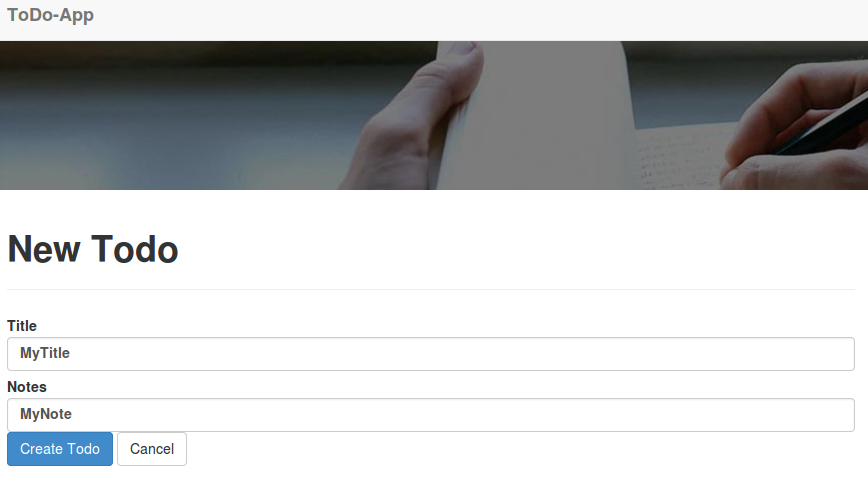
\includegraphics[width=0.49\textwidth]{img/newTodo.png}}
  \subfigure[Anzeigen eines Datensatzes]{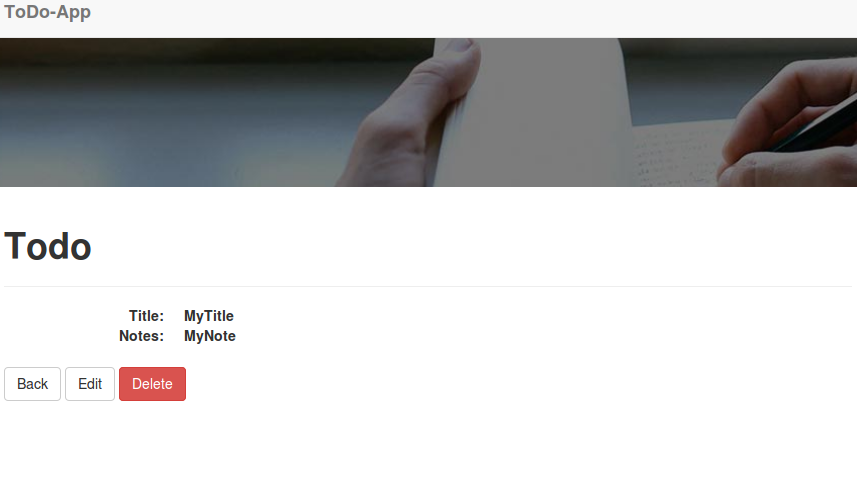
\includegraphics[width=0.49\textwidth]{img/showTodo.png}}
 \subfigure[Editieren eines Datensatzes]{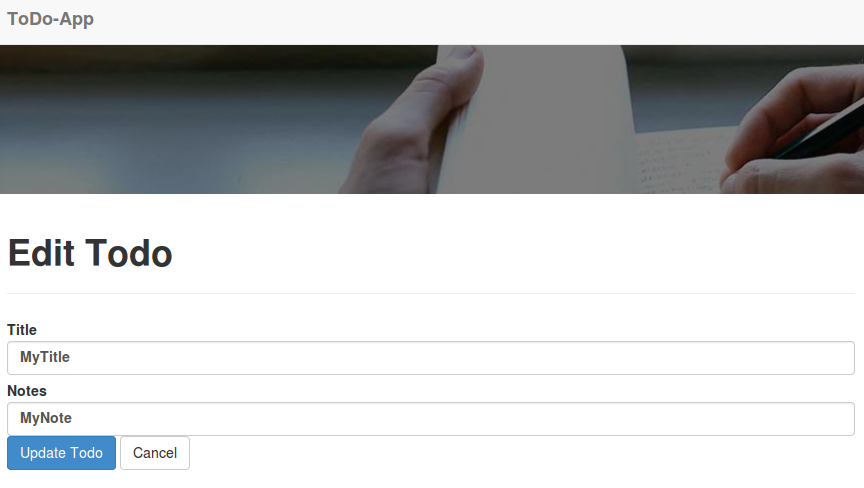
\includegraphics[width=0.49\textwidth]{img/editTodo.png}}
 \caption{Anlegen, editieren und anzeigen eines neuen Datensatzes}
  \label{fig:toDoApp}
\end{figure}


Zur besseren Lesbarkeit wurden die Testfälle im Listing \ref{lst:exportierteTestfaelle} überarbeitet, in ihrem grundlegendem Aufbau jedoch nicht verändert.\\
\begin{lstlisting}[caption={Exportierte Testfälle},label={lst:exportierteTestfaelle}]
  /**
  * Testfall legt einen neuen Datensatz an.
  */
  @Test
  public void testCreateNewRecord() {
    WebDriver driver = new FirefoxDriver();
    driver.get("http://localhost:3000/todos/new");
    driver.findElement(By.id("todo_title")).sendKeys("MyTitle");
    driver.findElement(By.id("todo_notes")).sendKeys("MyNote");
    driver.findElement(By.name("commit")).click();
  
    assertEquals("MyTitle", driver.findElement(By.id("title")).getText());
    assertEquals("MyNote", driver.findElement(By.id("note")).getText());
  }
  
  /**
  * Testfall legt einen neuen Datensatz an und editiert ihn.
  */
  @Test
  public void testEditRecord() {
    WebDriver driver = new FirefoxDriver();
    driver.get("http://localhost:3000/todos/new");
    driver.findElement(By.id("todo_title")).sendKeys("MyTitle");
    driver.findElement(By.id("todo_notes")).sendKeys("MyNote");
    driver.findElement(By.name("commit")).click();
    driver.findElement(By.linkText("Edit")).click();
    driver.findElement(By.id("todo_title")).clear();
    driver.findElement(By.id("todo_title")).sendKeys("MyTitleEdit");
    driver.findElement(By.id("todo_notes")).clear();
    driver.findElement(By.id("todo_notes")).sendKeys("MyNoteEdit");
    driver.findElement(By.name("commit")).click();
    
    assertEquals("MyTitleEdit", driver.findElement(By.id("title")).getText());
    assertEquals("MyNoteEdit", driver.findElement(By.id("note")).getText());
  }
  
\end{lstlisting}
Die in im Listing \ref{lst:exportierteTestfaelle} gezeigten Testfälle sind in ihren Abläufen recht ähnlich. Beide legen zunächst in der Anwendung einen neuen Datensatzan an. Die hierfür verwendete Logik ist dupliziert worden.\\
Das duplizieren von Code ist ein Problem, unter dem viele auf diesem Weg erzeugte Testfälle leiden. In den meisten Testabläufen finden sich wiederkehrende Aufgaben, die nicht nur von einem Testfall benötigt werden.
Selbst wenn sich die Abläufe zwischen den Testfällen stark unterscheiden werden Elemente, die von der Anwendung angeboten werden, in der Regel mehrmals benutzt. Das führt dazu, dass der Code zum adressieren dieser Felder in einer Vielzahl von Testfällen benutzt wird.\\
Als weiteres Problem haben Leotta et al. \cite{leotta_repairing_2013} eine starke Koppelung der Testfälle mit der Webanwendung genannt. Die Selektoren, die in den gezeigten Testfällen verwendet werden, um die Elemente der Webanwendung anzusteuern, sind direkt in den Code eingearbeitet. Änderungen an der Seitenstruktur der Anwendung, haben damit direkten Einfluss auf die Testfälle.
Obwohl sich die eigentliche Testfallspezifikation durch eine Änderung in der Seitenstruktur nicht ändert, müssen die Testfälle somit trotzdem überarbeitet werden.\\
Der duplizierte Code und der hohe Grad an Koppelung mit der Anwendung innerhalb der Testfälle bedingt, dass selbst kleine Änderungen in der zu testenden Anwendung, Korrekturen an vielen Stellen in den Testfällen notwendig macht.

\subsection{Manuell}
\label{sec:manuell}
Eine weitere Möglichkeit bildet das manuelle Erstellen der Testskripte. Für die Ausführung und Kommunikation mit der Anwendung, verwenden die manuell erstellten Skripte das selbe Toolset, wie die mittels \grq record-and playback\grq generierten und exportierten Testfälle. Analog zu den in Listing \ref{lst:exportierteTestfaelle} gezeigten Testfällen, wird auch bei diesen Skripten der Selenium WebDriver für die Kommunikation mit der Anwendung verwendet. Die Ausführung geschieht in der Regel ebenfalls über ein Unit-Fraemwork.\\
Im Vergleich zu den generierten Testfällen, ist das manuelle entwickeln der Testskripte aufwändiger.
Es bietet jedoch die Möglichkeit, den in Abschnitt \ref{sec:probleme_von_recorde_and_playback} genannten Problemen der \grq record-and playback\grq -Variante entgegenzuwirken.\\
Bei einem manuellen Ansatz kann von Anfang an auf eine wartbare und wiederverwertbare Struktur geachtet werden.
Als best practice hat sich zu diesem Zwecke das Page Object Design Pattern durchgesetzt.

\subsection{Page Object Pattern}
\label{sec:page_object_pattern}
Im Page Object Pattern wird versucht, die Funktionalität, welche die zu testende Anwendung anbietet, in einem objektorientierten Ansatz zu kapseln.
Alle Seiten der zu testenden Anwendung werden dazu als Kassen, sogenannten Page Objects, modelliert. Jede dieser Klassen verwaltet zentral alle Informationen, sowie die Funktionalität, die von der jeweils korrespondierenden Webseite angeboten wird. Die Hauptbestandteile eines Page Objects bilden Selenium-WebElemente. Im rahmen dieser Arbeit werden diese als \grq Elemente\grq\ bezeichnet. Elemente werden in den Page Objects meist als globale Variablen angeboten und bilden die Verbindung zu den HTML-Elementen welche auf der entsprechenden Webseite der Anwendung angeboten werden. Manche Elemente, wie beispielsweise Buttons, haben die Besonderheit, dass sie einen Seitenwechsel in der Webanwendung hervorrufen. Diese Elemente werden in der Arbeit als \grq Transitionen\grq\ bezeichnet. Transitionen werden analog zu den Elementen als globale Variablen geführt. Zusätzlich werden sie in den Page Objects meist in Form einer Methode abgebildet, die als Rückgabe das Page Object der entsprechenden Zielseite liefert. Funktionalität die von einer Seite angeboten wird, wird innerhalb eines Page Objects ebenfalls gekapselt in Methoden abgebildet.\\
Ein Page Objekt ist also eine objektorientierte Klasse, die als Interface für eine Seite der zu testenden Anwendung dient.
Sämtliche Interaktion mit der zu testenden Anwendung, geschieht über die in den Page Objekts angeboten Schnittstellen.
Änderungen an der Oberfläche der zu testenden Anwendung, haben so keinen direkten Einfluss mehr auf die Testfälle. Bei Änderungen an der Benutzeroberfläche muss nur noch Code an einer Stelle, innerhalb der Page Objekts, angepasst werden.\\
Um das Zusammenspiel zwischen Page Objekts und Testfall zu verdeutlichen, wurde der Test zum Anlegen eines neuen Eintrags aus Listing \ref{lst:exportierteTestfaelle} mit dem Page Object Pattern nachgebaut.\\
Der Testfall arbeitet mit zwei Seiten der Anwendung. Die Seiten wurden bereits in Abbildung \ref{fig:toDoApp} dargestellt. Für jede der beiden Seiten wird ein Page Object als Kommunikationsschnittstelle benötigt. 
Das Page Object CreatPage in Listing \ref{lst:poCreatePage} repräsentiert die Seite zum Anlegen eines neuen Datensatzes (Abbildung \ref{fig:toDoApp} a). Das Page Object ShowPage in Listing \ref{lst:poShowPage} repräsentiert die Seite zum Anzeigen eines Datensatzes (Abbildung \ref{fig:toDoApp} b).

\begin{lstlisting}[caption={Page Object CreatePage},label={lst:poCreatePage}]
  public class CreatePage extends BasePo {
		public final Control tfTodotitle = control(by.textField("todo_title"));
		public final Control tfTodonotes = control(by.textField("todo_notes"));
		public final Control bCreateTodo = control(by.button("commit"));
		
		public CreatePag(PageObject po) {
			super(po);
		}
		public ShowPage createEntry(String title, String note){
			tfTodotitle.sendKeys(title);
			tfTodonotes.sendKeys(note);
			bCreateTodo.click();
			return new ShowPage(this);
		}
  }
\end{lstlisting}  
\begin{lstlisting}[caption={Page Object ShowPage},label={lst:poShowPage}]  
  public class ShowPage extends BasePo {
		public final Control idTitle = control(by.id("title"));
		public final Control idNotes = control(by.id("note"));

		public ShowPage(PageObject po) {
			super(po);
		}
  }
\end{lstlisting}

Die Funktionalitäten, die von den jeweiligen Seiten angeboten werden, sind innerhalb des Page Objects gekapselt. Das Page Object CreatPage bietet beispielsweise die Eingabefelder für Titel und Note, sowie den Button zum Anlegen eines Datensatzes, als globale Objekte vom Typ Control an.\\
Die Klasse Control dient in den dargestellten Page Objekts als Wrapper für Selenium WebElementen. Control-Objekte sind also analog zu WebElementen zu verstehen.\\
Die Funktionalität zum Anlegen eines neuen Eintrags, die im späteren Testfall benötigt wird, bietet das Page Objekt CreatPage, als Methode \grq createEnty()\grq\ an.\\

Der Testfall in Listing \ref{lst:pageObjectTestfall} verwendet beide Page Objekts, um einen neuen Eintrag in der Anwendung anzulegen und zu überprüfen.\\


\begin{lstlisting}[caption={Page Object Testfall},label={lst:pageObjectTestfall}]  
  /**
  * Testfall legt einen neuen Datensatz an.
  */
 	@Test
	public void testCreateNewRecord(){
		CreatePage createPage = new CreatePage(po);
		ShowPage showPage = createPage.createEntry("MyTitle", "MyNote");

		assertEquals("MyTitle", showPage.idTitle.resolve().getText());
		assertEquals("MyNote", showPage.idNotes.resolve().getText());
	}

\end{lstlisting}

Im Gegensatz zum Testfall in Listing \ref{lst:exportierteTestfaelle}, ist es auf Grund des Page Object Pattern nicht mehr nötig, explizite Referenzen auf die Struktur der Seite in den Testfälle zu machen. Alle Details der Seite sind innerhalb der Page Objekts gekapselt. Der Testfall verwendet lediglich die im Page Object angebotene Funktionalität.


\subsubsection{Vorteile des Page Object Pattern}
\label{sec:vorteile_des_page_object_pattern}

Folgende Vorteile ergeben sich bei der Verwendung des Page Object Pattern, die auch in der Dokumentation von Selenium \cite{selenium_selenium_2015-2} angegeben werden:

\begin{enumerate}
\item Es gibt eine klare Trennung zwischen Testcode und seitenspezifischem Code, wie beispielsweise Elementadressierungen und Layout. \\ \\
Die Adressierung der Elemente ist nicht mehr über die gesamten Testfälle verteilt, sondern befindet sich an einem zentralen Ort, dem Page Object.
Die hohe Koppelung der Testfälle mit den Seiten der Anwendung, die Leotta et al. \cite{leotta_repairing_2013} als Problem genannt haben, kann somit überwunden werden.

\item Es gibt einen einzigen Ort für Elemente und Operationen die von einer Seite angeboten werden. \\ \\
Alle Informationen, die eine Seite der Anwendung betreffen, sind an einem zentralem Ort, dem Page Object gesammelt. Seitenspezifischer Code muss somit nicht mehr in den einzelnen Testfällen dupliziert werden. Die Funktionalitäten der Seite können über das entsprechende Page Object abgerufen werden.

\end{enumerate}

Die genannten Vorteile zeigen, dass Änderungen die an einer Seite durchgeführt werden, nur Auswirkungen an einer zentralen Stelle haben. Die Wartbarkeit der gesamten Testfälle wird so erhöht.
Leotta et al. unterstützen diese These mit einer Fallstudie \cite{leotta_repairing_2013}, in der sie eine herkömmliche Testsuite, mit einer Testsuite, die das Page Object Pattern implementiert, hinsichtlich ihrer Wartbarkeit verglichen haben.
Das Ergebnis dieser Studie hat gezeigt, dass die Zeit für die Wartung der Testfälle um ca. 65\% reduziert werden konnte. Die Anzahl der anzupassenden Codezeilen reduzierte sich um ca. 87\%.

\subsubsection{Probleme des Page Object Pattern}
\label{sec:probleme_des_page_object_pattern}

Den Vorteile des Page Object Pattern stehen allerdings auch Nachteile gegenüber. Die Komplexität des gesamten Testprojekts steigt. Testfälle können nicht mehr beliebig programmiert werden, sondern sind in den Kontext von Page Objekts zu stellen. Das erfordert tiefgründige Designentscheidungen. So ist beispielsweise zu klären, wie über die Page Objekts ein generischer Einstieg in die Anwendung angeboten werden kann, oder wie der WebDriver über mehrere Page Objekts und Testfälle hinweg verwaltet wird.\\
Darüber hinaus müssen die Page Objects zunächst initial entwickelt werden, bevor mit dem erstellen von Testfällen begonnen werden kann.\\
Verglichen mit einem herkömmlichen Ansatz, steigt mit der Verwendung des Page Object Pattern, daher der Aufwand zum Erstellen eines Testprojektes.\\
Wie in Kapitel \ref{sec:vorteile_des_page_object_pattern} bereits erwähnt, haben 
Leotta et al. \cite{leotta_repairing_2013} allerdings auch dargestellt, dass sich diese Investition durchaus lohnen kann.
